\documentclass[10pt, compress]{beamer}

\usetheme{m}

\usepackage{booktabs}
\usepackage[scale=2]{ccicons}
\usepackage{minted}

\usemintedstyle{pastie}

\title{Random number generation}
\subtitle{Quantitative Risk Management project work}
\date{}
\author{Silvia Baldisserotto, Maysa Jahanbani, \\ Claudia Pesci, Phan Ho Tan Phat, \\ Andrea Venuta}
\institute{Università degli Studi di Firenze - Finance and Risk Management}

\renewcommand{\theFancyVerbLine}{\sffamily \textcolor[rgb]{0.5,0.5,0.5}{\small \oldstylenums{\arabic{FancyVerbLine}}}}

\begin{document}

\maketitle

\begin{frame}[fragile]
  \frametitle{Random numbers}
  \begin{itemize}
  	\item Computer-generated numbers are \textit{pseudo-random}: deterministic and predictable
  	\item \textit{Quasi-random} numbers prevent potential lack of equidistributedness
  	\item \textbf{Definition.} \textit{(sample)} a sequence of number is called a \textit{sample from the distribution $F$}
  	  if the numbers are independent realizations of a random variable with distribution function $F$
	\item Uniform deviates: samples from $\sim \mathcal{U}  \left[ 0, 1 \right] $
	\item Normal deviates: samples from $\sim \mathcal{N}  \left( 0, 1 \right) $
	\item Drawing uniform deviates is the basis of random number generation
  \end{itemize}
\end{frame}

\begin{frame}[fragile]
  \frametitle{Linear congruential generators}
  	\begin{itemize}
  	  \item $N_0$ is chosen arbitrarily
  	  \item $N_i = (aN_{i-1} + b)\ \text{mod}\ M$ for $i > 0$
  	\end{itemize}
\end{frame}

\begin{frame}[fragile]
  \frametitle{Quality of generators}
  Requirements:
  \begin{enumerate}
  	\item Large period: small set of numbers makes the outcome easier to predict (choose M as large as possible)
  	\item Statistical tests to verify that the distribution is the intended one
  	  \begin{itemize}
  	  	\item Comparison of sample mean and variance $\mu,\ \sigma^2$ with desired values
  	  	\item Correlation between sample values
  	  	\item Quality of approximation of the distribution
  	  \end{itemize}
     \item Distribution in higher dimensional spaces: lattice structure
  \end{enumerate}
\end{frame}

\begin{frame}[fragile]
  \frametitle{Random vectors and lattice structure}
  \begin{itemize}
  	\item Sequences of random numbers can be arranged in $m$-dimensional vectors
  	\item The vectors lie on a number of parallel $(m-1)$-dimensional hyperplanes
  	\item The ideal condition is that the number of parallel hyperplanes is maximized:
  	  number of hyperplanes is a measure of equidistributedness
  	\item Family of parallel lines in the $(U_{i-1},U_i)$-plane \[
  		z_0 U_{i-1} +z_1 U_i = c + \frac{z_1 b}{M} \quad \text{where} \quad c := N_{i-1}\frac{z_0 + az_1}{M} - z_1 k
  	  \] for each tuple $(z_0,z_1)$ and for all $c$s.
  \end{itemize}
\end{frame}

\begin{frame}[fragile]
  \frametitle{Random vectors and lattice structure}
  immagini qui
\end{frame}

\begin{frame}[fragile]
  \frametitle{Inversion and transformation methods}
  \begin{itemize}
  	\item Inversion and transformation methods generate numbers distributed according to
  	  an arbitrary distribution from uniformly distributed samples
  \end{itemize}
\end{frame}

\begin{frame}[fragile]
	\frametitle{Implementations - Linear Congruential Generator}
	\begin{columns}[t]
		\begin{column}{5cm}
	
			\begin{minted}[fontsize=\small,linenos]{matlab}
function [ rn ] = LCG( x ) 

  if(nargin == 0)
    x = 1;
  end
  
  rn = zeros(x,1);
  
  for i = 1:x
    rn(i) = LCGstep();
  end

end
			\end{minted}
		\end{column}
		\begin{column}{5cm}
			\begin{minted}[fontsize=\small,linenos,firstnumber=14]{matlab}
function [ rnStep ] = LCGstep()

  persistent seed;
  M = 244944;
  a = 1597;
  b = 51749;
  
  if(isempty(seed))
    seed = 0;
  end
  
  seed = mod(seed * a + b, M);
  
  rnStep = seed / M;

end
			\end{minted}
		\end{column}
	\end{columns}
\end{frame}

\begin{frame}[fragile]
	\frametitle{Implementations - Box-Muller method}
	\begin{minted}[fontsize=\small,linenos]{matlab}
function [ Z ] = BoxMuller( x )

  if(nargin == 0)
    x = 1;
  end

  U = rand(x, 2);
  
  theta = 2 .* pi .* U(:, 2);
  rho   = sqrt( -2 .* log( U(:, 1) ) );
  
  Z = [ rho .* cos(theta), rho .* sin(theta) ];

end
	\end{minted}
\end{frame}

\begin{frame}[fragile]
	\frametitle{Implementations - Marsaglia polar algorithm}
	\begin{minted}[fontsize=\small,linenos]{matlab}
function [ Z ] = Marsaglia( x )

  if(nargin == 0)
    x = 1;
  end

  Z = zeros(x,2);
  
  for i = 1 : x
    W = 1;  V = [ 1, 1 ];
    while not (W < 1)
      V = 2 * rand(1, 2) - 1;
      W = V(1) .^ 2 + V(2) .^ 2;
    end
    
    Z(i, :) = V .* sqrt(-2 * log(W) / W);
  end
end
	\end{minted}
\end{frame}

\begin{frame}[fragile]
	\frametitle{Plots - Univariate methods}
	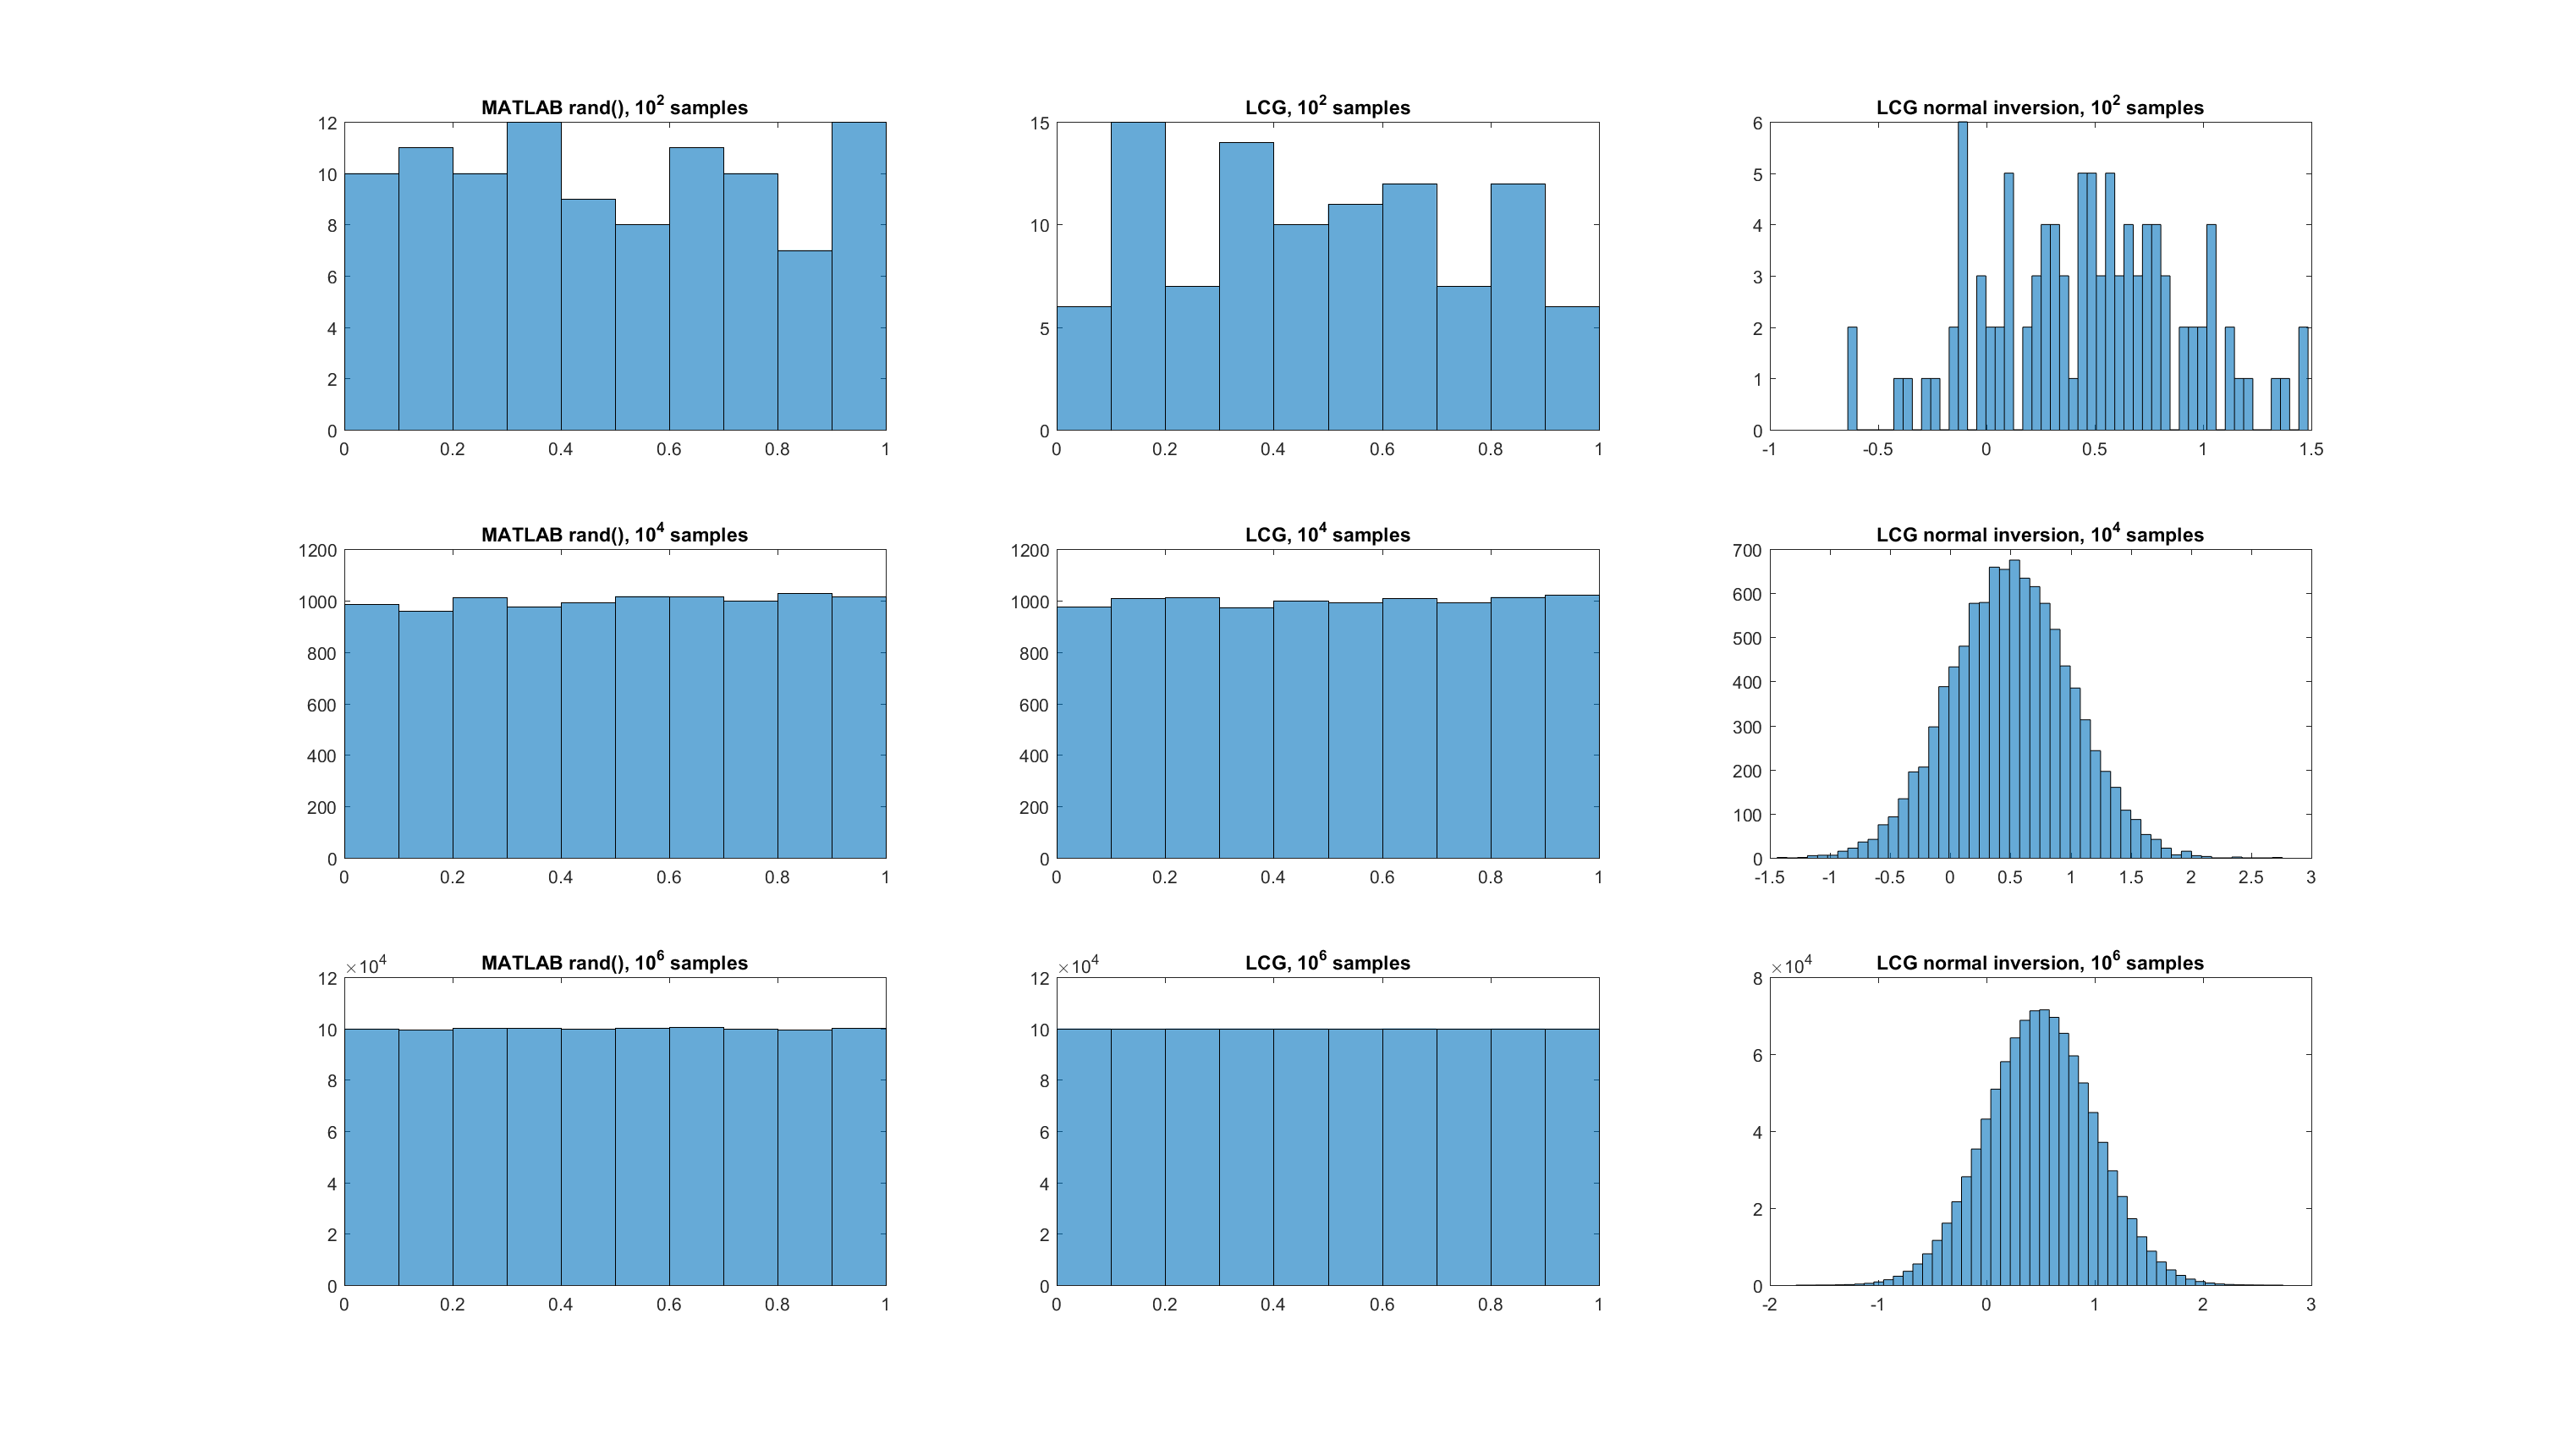
\includegraphics[width=\textwidth, trim=70mm 80mm 70mm 20mm]{../univariate.eps}
\end{frame}

\begin{frame}[fragile]
	\frametitle{Plots - Bivariate methods}
	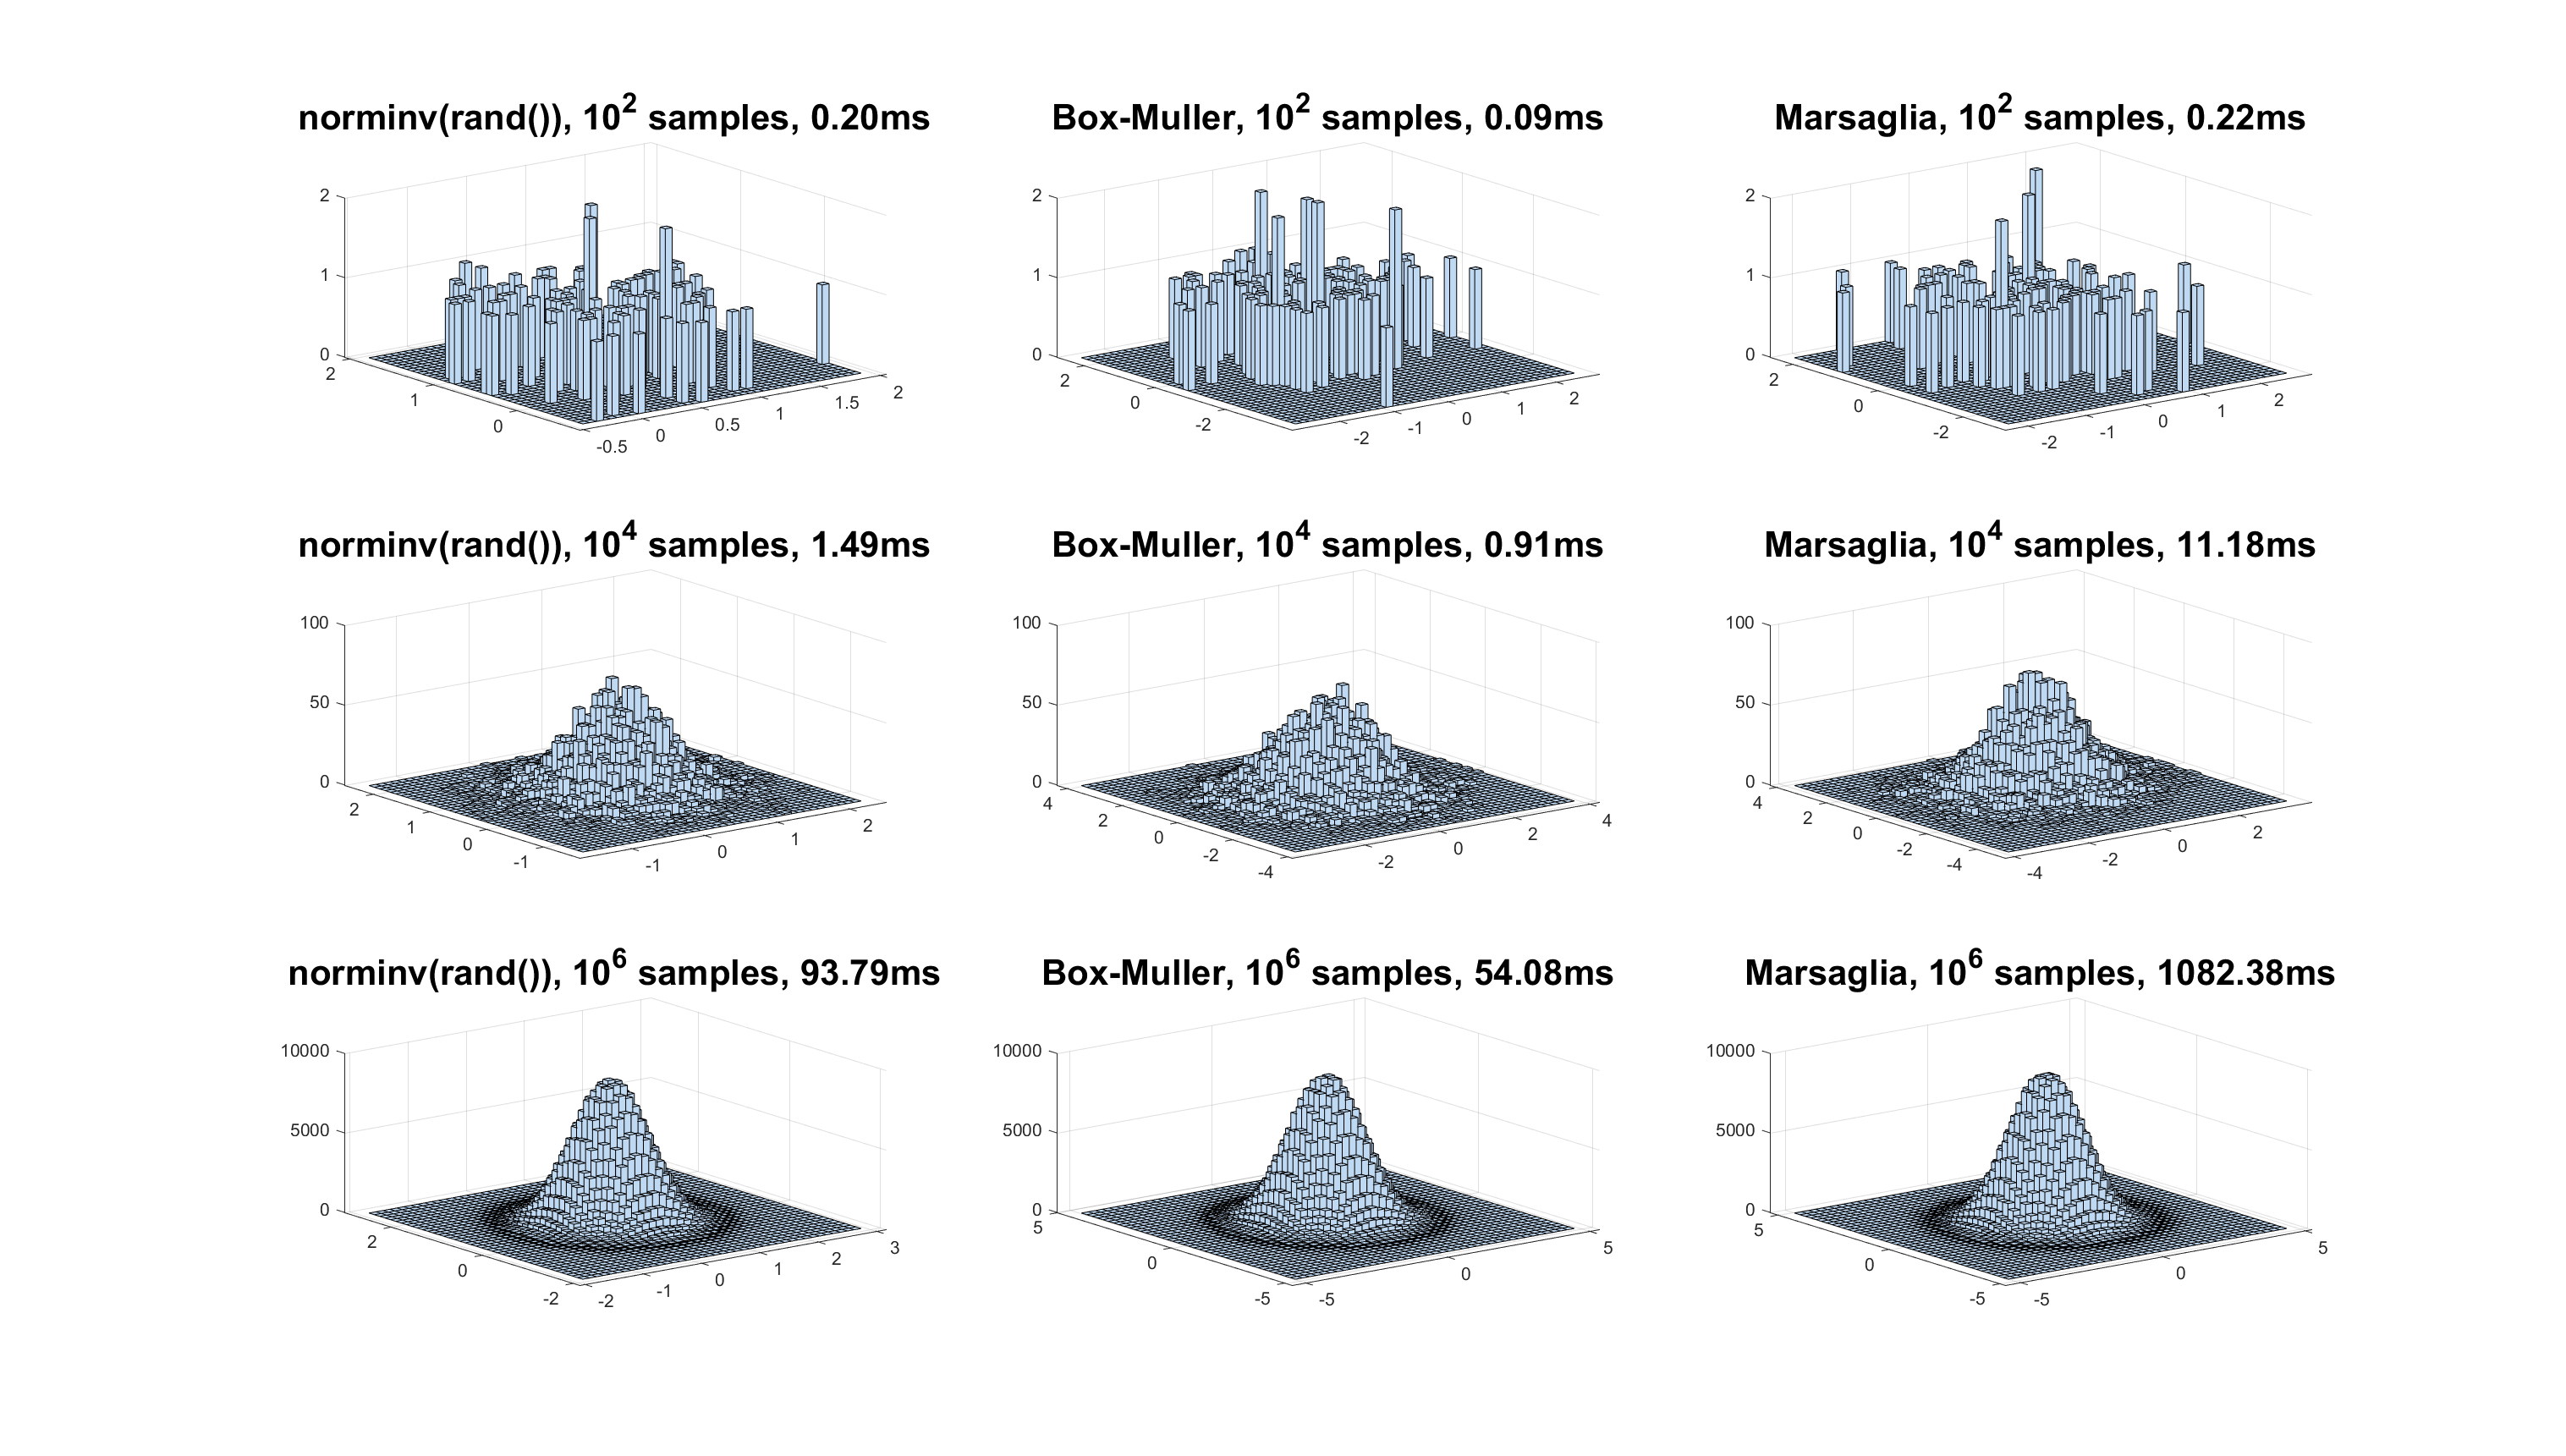
\includegraphics[width=\textwidth, trim=70mm 80mm 70mm 20mm]{../bivariate.eps}
\end{frame}

\end{document}
